\documentclass[tikz,border=10pt]{standalone}
\usepackage{tikz}
\usetikzlibrary{arrows.meta,calc}
\begin{document}
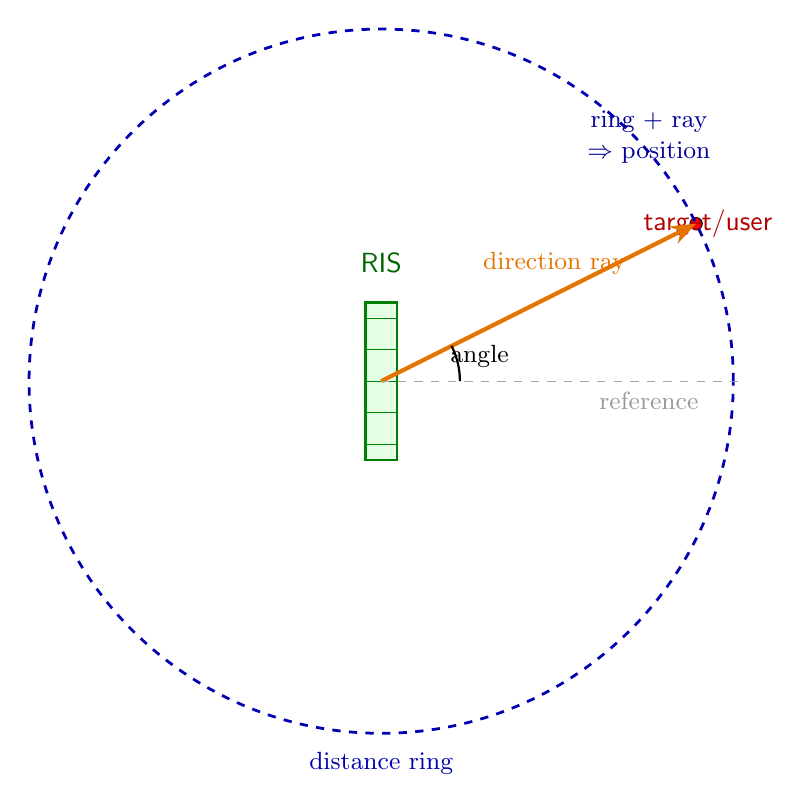
\begin{tikzpicture}[font=\sffamily,>=Stealth]
  % RIS panel at origin
  \draw[fill=green!10, draw=green!50!black, line width=1pt] (-0.2,-1.0) rectangle (0.2,1.0);
  \foreach \y in {-0.8,-0.4,0.0,0.4,0.8} {
    \draw[green!50!black] (-0.2,\y) -- (0.2,\y);
  }
  \node[align=center, text=green!40!black] at (0,1.5) {RIS};

  % user point
  \coordinate (user) at (4.0,2.0);
  \draw[fill=red] (user) circle (2.2pt);
  \node[align=left, text=red!70!black] at (4.15,2.0) {target/user};

  % distance ring
  \draw[dashed, blue!70!black, line width=1pt] (0,0) circle (4.472);
  \node[blue!70!black, font=\small] at (0,-4.85) {distance ring};

  % direction ray
  \draw[-{Stealth[length=3.2mm]}, orange!90!black, line width=1.5pt] (0,0) -- (user);
  \node[orange!90!black, font=\small, align=left] at (2.2,1.5) {direction ray};

  % angle arc
  \draw[thick] (1.0,0) arc [start angle=0, end angle=26.6, radius=1.0];
  \node[font=\small] at (1.25,0.32) {angle};

  % helper horizontal line
  \draw[dashed, gray!70] (0,0) -- (4.6,0);
  \node[gray!80, font=\small] at (3.4,-0.25) {reference};

  \node[align=center, font=\small, text=blue!60!black] at (3.4,3.1) {ring + ray\\$\Rightarrow$ position};
\end{tikzpicture}
\end{document}
